\section{Verifying ranked group fairness for a single protected group. }
\label{sec:adjustment-binomial}
\begin{table}[t]
	\caption{Time complexity for all algorithms without pre-computed results.\label{tbl:time-space-binom}}
	\vspace{-4mm}
	\scalebox{0.75}{
		\begin{tabular}{lll}
			\toprule
			\textbf{Algorithm} & \textbf{Time Complexity} & \textbf{Space Complexity}\\
			\midrule
			\rowcolor[HTML]{C0C0C0}
			\algoMtable & $\mathcal{O}(k) \cdot \mathcal{O}(inverseBinomialCDF(p,k,\alpha))$ & $\mathcal{O}(k)$ \\
			\algoRecursive & $\mathcal{O}(\algoMtable) + \mathcal{O}(\prod_{j=1}^{m(k)}b(j) \cdot O(\texttt{binomPDF}))$ & $\mathcal{O}(k)$ \\
			\rowcolor[HTML]{C0C0C0}
			\algoBinomBinary & $\mathcal{O}(\log{}k^2) \cdot (\mathcal{O}(\algoRecursive))$ & $\mathcal{O}(k)$  \\
			\bottomrule
		\end{tabular}
	}
\end{table}

%
For binomial distributions, i.e. where only one protected and one non-protected group is present, the inverse CDF can be stored as a simple table. Analogous to the multinomial case, we will call such a table \textit{mTable}.
%
Table~\ref{tbl:ranked_group_fairness_table} shows an example of such a pre-computed table with different $ k $ and $ p $, using $\alpha=0.1$.
%
For instance, for $p=0.5$ we see that at least 1 candidate from the protected group is needed in the top 4 positions, and 2 protected candidates in the top 7 positions.

\begin{table}[t!]
	\caption{Example values of $m_{\alpha,p}(k)$, the minimum number of candidates in the protected group that must appear in the top $k$ positions to pass the ranked group fairness criteria with $\alpha=0.1$ in a binomial setting.}
	\vspace{-3mm}
	\label{tbl:ranked_group_fairness_table}
	\small\begin{tabular}{r|cccccccccccc}
		\diaghead{some text}%
		{p}{k}&
		% & \multicolumn{10}{c}{k} \\
		1 & 2 & 3 & 4 & 5 & 6 & 7 & 8 & 9 & 10 & 11 & 12 \\ \midrule
		0.1      & 0 & 0 & 0 & 0 & 0 & 0 & 0 & 0 & 0 & 0  &  0 &  0 \\
		0.2      & 0 & 0 & 0 & 0 & 0 & 0 & 0 & 0 & 0 & 0  &  1 &  1 \\
		0.3      & 0 & 0 & 0 & 0 & 0 & 0 & 1 & 1 & 1 & 1  &  1 &  2 \\
		0.4      & 0 & 0 & 0 & 0 & 1 & 1 & 1 & 1 & 2 & 2  &  2 &  3 \\
		0.5      & 0 & 0 & 0 & 1 & 1 & 1 & 2 & 2 & 3 & 3  &  3 &  4 \\
		0.6      & 0 & 0 & 1 & 1 & 2 & 2 & 3 & 3 & 4 & 4  &  5 &  5 \\
		0.7      & 0 & 1 & 1 & 2 & 2 & 3 & 3 & 4 & 5 & 5  &  6 &  6 \\
		\bottomrule
	\end{tabular}
\end{table}

Figure~\ref{fig:why-adjustment-is-needed-binomial} shows, even though the slope is not as steep as in the multinomial case, that we still need a correction for $\alpha$.
%
In the following section, we will show that the special case of one protected group offers new possibilities for verifying ranked group fairness. A key improvement is that we can calculate the exact probability with which a fair ranking gets rejected by the ranked group fairness test in the binomial setting. Note that in the multinomial case, we can only estimate this probability by testing 10,000 rankings. This will not only make the resulting $\alphaadj$ the best possible, it will also result in a more efficient binary search for it. 
%
In section \ref{subsubsec:adjustment-binomial} we introduce the necessary notation for the binomial case and describe how we calculate the exact probability that a fair ranking gets rejected (hence accepted) by the ranked group fairness test with one protected group.
In section \ref{subsec:finding-mtable} we show that we can divide the continuum of possible $\alpha$ values in discrete parts in order to be able to apply efficient binary search for the most accurate $\alphaadj$
%
%This figure is generated by simulation, generating rankings using the process described above and showing the probability of those rankings being rejected by our ranked group fairness test with $\alphaadj=0.1$.
%
%The figure suggests that depending on $k$ we would need to change the value of $\alpha$ if we want to achieve a rejection rate of $0.1$.

\begin{figure}[h]
	\centering
	{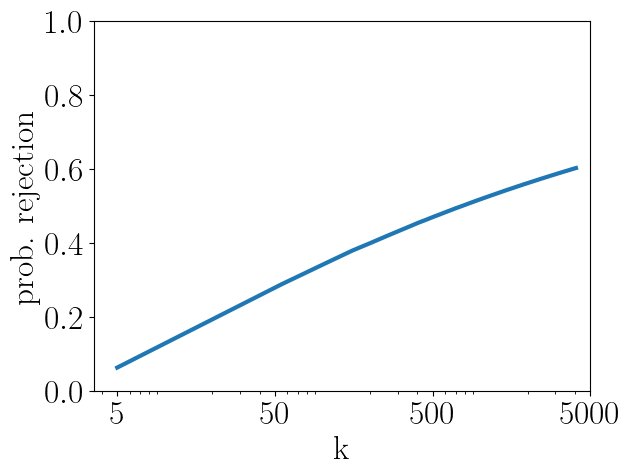
\includegraphics[width=.48\textwidth]{pics/failProbPlotBinom.png}}
	\caption{
		Probability that a fair ranking created by a Bernoulli process with $p=0.5$ fails the ranked group fairness test.\label{fig:why-adjustment-is-needed-binomial}
		%
		Experiments on data generated by a simulation, showing the need for multiple tests correction.
		%
		The data has: one protected group, with a ranking created by  a Bernoulli process (Fig.~\ref{fig:why-adjustment-is-needed-binomial}); and two protected groups, with a ranking created by a multinomial process (Fig.~\ref{fig:why-adjustment-is-needed-multinomial}).
		%
		Rankings should have been rejected as unfair at a rate $\alpha = 0.1$.
		%
		However, we see that the rejection probability increases with $k$.
		%
		Note the scale of $k$ is logarithmic.}
	\label{fig:need-for-model-adjustment}
\end{figure}

\subsection{Success Probability for One Protected Group}\label{subsubsec:adjustment-binomial}

The probability that a fair ranking, created by the process of~\citet{yang2016measuring}, passes the ranked group fairness test (success probability) with parameters $(p,\alpha)$ can be computed as follows:
%
Let $m(k) = m_{\alpha,p}(k) = F^{-1}(k,p,\alpha)$ be the number of protected elements required up to position $k$.
%
Let $\minv(i) = k$ s.t. $m(k) = i$ be the position at which $i$ protected elements are required.
%
Let $b(i) = \minv(i) - \minv(i-1)$ (with $\minv(0) = 0$) be the size of a ``block,'' that is, the gap between one increase and the next in $m(\cdot)$.
%
We call the $k$-dimensional vector $(m(1), m(2), \ldots , m(k))$ a \emph{mTable}.
%
An example is shown on Table~\ref{tbl:05:example_blocks}.
%
\begin{table}[h]
	\centering
	\begin{tabular}{cccccccccccccc}\toprule
		$k$    & 1 & 2 & 3 & \textbf{{4}} & 5 & 6 & \textbf{7} & 8 & \textbf{9} & 10 & 11 & \textbf{12} \\
		\midrule
		$m(k)$ & 0 & 0 & 0 & \multicolumn{1}{c|}{1} & 1 & 1 & \multicolumn{1}{c|}{2} & 2 & \multicolumn{1}{c|}{3} & 3  & 3  & \multicolumn{1}{c}{4}\\
		Inverse   & \multicolumn{4}{c|}{$\minv(1)=4$}
		& \multicolumn{3}{c|}{$\minv(2)=7$}
		& \multicolumn{2}{c|}{$\minv(3)=9$}
		& \multicolumn{3}{c}{$\minv(4)=12$}\\
		Blocks       & \multicolumn{4}{c|}{$b(1)=4$}
		& \multicolumn{3}{c|}{$b(2)=3$}
		& \multicolumn{2}{c|}{$b(3)=2$}
		& \multicolumn{3}{c}{$b(4)=3$}\\
		\bottomrule
	\end{tabular}
	\caption[Example of different block sizes]{Example of $m(\cdot)$, $\minv(\cdot)$, and $b(\cdot)$ for $p=0.5, \alpha=0.1$.}
	\label{tbl:05:example_blocks}
\end{table}

\noindent Furthermore let
\begin{equation}
	\label{eq:05:combinations}
	I_{m(k)} = \{ v = (i_1, i_2, \ldots, i_{m(k)}): \forall \ell' \in \lbrace 1,\ldots,m(k) -1 \rbrace, 0 \le i_{\ell'} \le b(\ell') \wedge \sum_{j=1}^{\ell'} i_j \ge \ell' \}
\end{equation}
%
represent all possible ways in which a fair ranking\footnote{Note that we do not consider rankings of size 0, which always pass the test.} generated by the method of \citet{yang2016measuring} can pass the ranked group fairness test, with $i_j$ corresponding to the number of protected elements in block $j \; (\text{with } 1 \le j \le k)$.
%
As an example consider again Table~\ref{tbl:05:example_blocks}: the first block contains four positions, i.e. $b(1)=4$ and this block passes the ranked group fairness test, if it contains at least one protected candidate.
%
It also passes the test, if it contains more protected candidates, hence $i_1 \in \{1, 2, 3, 4\}$.

The probability of considering a ranking of $k$ elements (i.e. $m(k)$ blocks) unfair, is:
\begin{equation}
	\label{eq:05:failureProb}
	1 - \sum_{v \in I_{m(k)}} \prod_{j=1}^{m(k)} f(v_j; b(j), p)
\end{equation}
%
\noindent where $f(x;b(j),p) = Pr(X = x)$ is the probability density function (pdf) of a binomially distributed variable $X \sim Bin(b(j), p)$.
%
However, if calculated naively this expression is intractable because of the large number of combinations in $I_{m(k)}$.

\setlength{\textfloatsep}{2pt}% Remove \textfloatsep
\begin{algorithm}[t!]
	\caption{Algorithm \algoRecursive computes the probability, that a given mTable accepts a fair ranking (see right term of Eq.~\ref{eq:05:failureProb}).}
	\label{alg:05:successProb} % But whenever possible refer to this algo. by name not number
	\small
	\AlgInput{
		$\texttt{b[]}$ list of block lengths (Table~\ref{tbl:05:example_blocks}, 3rd line);\\ 
		$\texttt{maxProtected}$ the sum of all entries of $\texttt{b[]}$;\\
		$\texttt{currentBlockIndex}$ index of the current block; \\
		$\texttt{candidatesAssigned}$ number of protected candidates assigned for the current possible solution; \\
		$p$, the expected proportion of protected elements.}
	\AlgOutput{The probability of accepting a fair ranking.}
	
	\If{$\texttt{b[].length} = 0$}{
		\Return{$1$}
	}
	\tcp{we need to assign at least one protected candidate to each block}
	$\texttt{minNeededThisBlock} \leftarrow \texttt{currentBlockIndex} - \texttt{candidatesAssigned}$\\
	\tcp{if we already assigned enough candidates, minNeededThisBlock = 0 (termination condition for the recursion)}
	\If{$\texttt{minNeededThisBlock} < 0$}{
		$\texttt{minNeededThisBlock} \leftarrow 0$
	}
	$\texttt{maxPossibleThisBlock} \leftarrow \textit{argmin}(\texttt{b[0]}, \texttt{maxProtected})$ \\
	$\texttt{assignments} \leftarrow 0$ \\
	$\texttt{successProb} \leftarrow 0$ \\
	\tcp{sublist without the first entry of $\texttt{b[]}$}
	$\texttt{b\_new[]} \leftarrow \textit{sublist}(\texttt{b[]}, 1, \texttt{b[].length})$ \label{algoline:05:suffixes}\\
	$\texttt{itemsThisBlock} \leftarrow \texttt{minNeededThisBlock}$\\
	\While{$\texttt{itemsThisBlock} \leq \texttt{maxPossibleThisBlock}$}{
		$\texttt{remainingCandidates} \leftarrow \texttt{maxProtected} - \texttt{itemsThisBlock}$ \\
		$\texttt{candidatesAssigned} \leftarrow \texttt{candidatesAssigned} + \texttt{itemsThisBlock}$ \\
		\tcp{each recursion returns the success probability of \emph{all possible ways} to fairly rank protected candidates after this block}
		$\texttt{suffixSuccessProb} \leftarrow \textsc{\algoRecursive} ( $ \\ \pushline $ \texttt{remainingCandidates},\texttt{b\_new[]}, \texttt{currentBlockIndex} + 1,$ \\ $ \texttt{candidatesAssigned})$ 
		\label{algoline:05:recursion}\\
		\popline $\texttt{totalSuccessProb} \leftarrow \texttt{totalSuccessProb} \; + $ \\ \pushline $ \textsc{PDF}(\texttt{maxPossibleThisBlock}, \texttt{itemsThisBlock}, p) \; \cdot $ \\ $ \texttt{suffixSuccessProb}$ \label{algoline:05:pdf}\\
		\popline $\texttt{itemsThisBlock} \leftarrow \texttt{itemsThisBlock} + 1$\\
	}
	\Return{probability of accepting a fair ranking: $\texttt{totalSuccessProb}$ }
\end{algorithm}
We therefore propose Algorithm~\ref{alg:05:successProb}, which computes the probability that a fair ranking passes the ranked group fairness test (i.e. the right term of Equation~\ref{eq:05:failureProb}) \emph{recursively}.
%
%With this algorithm however, we have to account for an important pitfall: we may choose a combination of $k, p, \alpha$ where the last block ``reaches beyond'' $k$.
%
%Consider again Table~\ref{tbl:05:example_blocks} with $k=8, \minpro$p=$0.5, \alpha=0.1$: the second block reaches until position 7, while the third block reaches until position 9.
%
%If we cut off the mTable at $k=8$ to adjust the significance level, the last block reaches beyond $k$ which is to position 9.
%
%\meike{Inwiefern macht der neue Algorithmus das Problem mit aufgebrochenen Blöcken besser?}
%To account for that t
The algorithm breaks the vector $v = (i_1, i_2, \ldots ,i_{\ell})$ of Equation~\ref{eq:05:combinations} into a \textit{prefix} and a \textit{suffix} (Alg.~\ref{alg:05:successProb}, Line~\ref{algoline:05:suffixes}).
%
We call $i_1$ the \textit{prefix} of $(i_2, \ldots, i_{\ell})$, and $(i_2, \ldots, i_{\ell})$ the \textit{suffix} of $i_1$.
%
The algorithm starts with a prefix and calculates all possible suffixes, that pass the ranked group fairness test, recursively (Line~\ref{algoline:05:recursion}).
%
Consider the following example: for the first prefix $i_1 = 1$ the algorithm computes all possible suffixes, where we rank exactly one protected candidate in the first block.
%
For this prefix $i_1$ combined with each possible suffix $v \setminus i_1$ we calculate $\prod_{j=1}^{m(k)} f(v_j; b(j), p)$ (Line~\ref{algoline:05:pdf}), which is the probability that one particular instance of $v$ passes the ranked group fairness test (for short, we refer to it as the ``success probability'').
%
In the next recursion the prefix is $i_1=1, i_2 =1$ and the algorithm computes all possible suffixes, i.e. all rankings where we rank exactly one protected candidates in the first block and one protected candidate in the second block, and the respective success probabilities.
%
This procedure continues for $m(k)$ iterations.
%
After that the entire procedure starts again with $i_1=2$ and is repeated until the maximum number of protected candidates is reached, in our case $b(1)=4$.
%
All intermediate success probabilities are added up (Line~\ref{algoline:05:pdf}) to the total success probability of the mTable that was created with the given setting of $k, p, \alpha$.

Note that there are at most $\prod_{j=1}^{m(k)}b(j)$ possible combinations to distribute the protected candidates within the blocks.
%
Furthermore many $v \in I_{m(k)}$ share the same prefix and hence have the same probability density value for these prefixes.
%
To reduce computation time the algorithm stores the binomial probability density value for each prefix in a hash map with the prefix as key and the respective pdf as value.
%
Thus the overall computational complexity becomes $O(\prod_{j=1}^{m(k)}b(j) \cdot O(\texttt{binomPDF}))$.

\subsection{Finding the Correct mTable}\label{subsec:finding-mtable}
To find the correct mTable, that is the mTable with an overall acceptance probability of $1-\alpha$, we propose Algorithm~\ref{alg:05:binarySearch} that takes  parameters $k, p, \alphaadj$ as input.
%
%We use Algorithm~\ref{alg:05:successProb} to determine the adjusted significance level $\alphaadj$ for the ranked group fairness test, such that the overall acceptance probability for the mTable with parameters $k, p, \alphaadj$ becomes $1-\alpha$.
%
It sequentially creates mTables (recall that these are $k$-dimensional vectors of the form $(m(1), m(2), \ldots , m(k))$) for different values of $\alphaadj$, and then calls Algorithm~\ref{alg:05:successProb} to calculate their success probability until it finds the correct mTable with overall failure probability $\alpha$ . Our goal is to use binary search to select possible candidates for $\alphaadj$ systematically.

\begin{algorithm}[t!]
	\caption{Algorithm \algoBinomBinary calculates the corrected significance level $\alpha_c$ and the mTable $m_{\alpha_c , k, p)}$ with an overall probability $\alpha$ of rejecting a fair ranking.}
	\label{alg:05:binarySearch} % But whenever possible refer to this algo. by name not number
	\footnotesize
	\AlgInput{$k$, the size of the ranking to produce; $p$, the expected proportion of protected elements; $\alpha$, the desired significance level.}
	\AlgOutput{$\alphaadj$ the adjusted significance level; \texttt{m\_{adjusted}} the adjusted mTable}
	\AlgComment{initialize all needed variables}
	\texttt{aMin $\leftarrow$ 0};
	\texttt{aMax $\leftarrow \alpha$ };
	\texttt{aMid} $\leftarrow \frac{(\texttt{aMin + aMax})}{2}$ \\
	\texttt{m\_min} $\leftarrow$ \texttt{constructMTable(k,p,aMin)}; 
	\texttt{m\_max} $\leftarrow$ \texttt{constructMTable(k,p,aMax)}; \\
	\texttt{m\_mid} $\leftarrow$ \texttt{constructMTable(k,p,aMid)} \\
	\texttt{maxMass} $\leftarrow$ \texttt{m\_max.getMass()};
	\texttt{minMass} $\leftarrow$ \texttt{m\_min.getMass()};
	\texttt{midMass} $\leftarrow$ \texttt{m\_mid.getMass()}\\
	
	\While{\texttt{minMass} $<$ \texttt{maxMass} AND \texttt{m\_mid.getFailProb()} $\neq \alpha$ }{
		\If{\texttt{m\_mid.getFailProb()} $< \alpha$}{
			\texttt{aMin} $\leftarrow$ \texttt{aMid}
			\texttt{m\_min} $\leftarrow$ \texttt{constructMTable(k,p,aMin)} \\
		}
		\If{\texttt{m\_mid.getFailProb()} $> \alpha$}{
			\texttt{aMax} $\leftarrow$ \texttt{aMid} \\
			\texttt{m\_max} $\leftarrow$ \texttt{constructMTable(k,p,aMax)} \\
		}
		\texttt{aMid} $\leftarrow \frac{(\texttt{aMin + aMax})}{2}$ \\
		\tcp{stop criteria if midMass equals maxMass or midMass equals minMass}
		\If{\texttt{maxMass - minMass == 1}}{
			\texttt{minDiff} $\leftarrow |$\texttt{m\_min.getFailProb() - }$\alpha|$ \\
			\texttt{maxDiff} $\leftarrow |$\texttt{m\_max.getFailProb() - }$\alpha|$ \\
			\tcp{return the $\alpha_c$ which has the lowest difference from the desired significance}			
			\If{\texttt{minDiff} $<$ \texttt{maxDiff}}{
				\Return{\texttt{aMin, m\_min}}
			}
			\Else{
				\Return{\texttt{aMax, m\_max}}
			}
		}
		\tcp{stop criteria if midMaxx is exactly the mass between minMass and maxMass}
		\If{\texttt{maxMass - midMass == 1} AND \texttt{midMass - minMass == 1}}{
			\texttt{minDiff} $\leftarrow |$\texttt{m\_min.getFailProb() - }$\alpha|$ \\
			\texttt{maxDiff} $\leftarrow |$\texttt{m\_max.getFailProb() - }$\alpha|$ \\
			\texttt{midDiff} $\leftarrow |$\texttt{m\_mid.getFailProb() - }$\alpha|$ \\
			\tcp{return the $\alpha_c$ which has the lowest difference from the desired significance}			
			\If{\texttt{midDiff} $\leq$ \texttt{maxDiff} AND \texttt{midDiff} $\leq$ \texttt{minDiff}}{
				\Return{\texttt{aMid, m\_mid}}
			}
			\If{\texttt{minDiff} $\leq$ \texttt{midDiff} AND \texttt{minDiff} $\leq$ \texttt{maxDiff}}{
				\Return{\texttt{aMin, m\_min}}
			}
			\Else{
				\Return{\texttt{aMax, m\_max}}
			}
		}
	}
	\Return{\texttt{aMid, m\_mid}}
\end{algorithm}
%\note[ChaTo]{Perhaps the definition of the mass of an mTable can wait a few more paragraphs, until you need it.}
However, to be able to do binary search, we need a discrete measure for the $\alpha$ space to search on. Otherwise, if we would perform binary search only on the interval $[0,1]$, the search would never stop.
%
Furthermore we only want to consider mTables with certain properties, which we define in the following paragraph. 
%
A $k$-dimensional vector (e.g. $(0,0,1,2,3)$) has to have two properties in order to constitute a mTable, rather than just a vector of natural numbers: it has to be \emph{valid} and \emph{legal}.
%
\begin{definition}[Valid mTable]
	\label{def:05:valid-mtable}
	The $\text{mTable}_{p,k,\alpha}=(m(1) , m(2) , \ldots , m(k))$ is \emph{valid} if and only if, $m(i) \leq m(j)$ for all $i,j \in \lbrace 1, \ldots, k \rbrace$ with $i < j$ and $m(i)=n \Rightarrow m(i+1) \leq n+1$.
\end{definition}
\noindent It is easy to see that many valid mTables exist.
%
They correspond to all $k$-dimensional arrays with integers monotonically increasing by array indices.
%
However we only want to consider those valid mTables for our ranked group fairness test that have been created by the statistical process in~\citet{yang2017measuring}.
%
We call these \textit{legal mTables}.
%
\begin{definition}[Legal mTable]
	\label{def:05:legal-mtable}
	A $\text{mTable}_{p,\alpha,k}$ is \textit{legal} if and only if there exists a $p,k,\alpha$ such that
	$\texttt{constructMTable}(p,k,\alpha)=\text{mTable}_{p,\alpha,k}$.
\end{definition}
%
\begin{definition}[constructMTable]
	\label{def:05:construct-mtable-single-test}
	For $p\in [0,1], k \in \mathbb{N}, \alpha \in [0,1]$ we define a function to construct a mTable from input parameters $p, k, \alpha$ according to \cite{yang2017measuring}.
	
	\noindent$\texttt{constructMTable} : \\ (0,1) \times \mathbb{N} \times [0,1] \longrightarrow \lbrace (m(1) ,\ldots, m(k)): m(i) = F^{-1}(i,p,\alpha), \, i = \{1,\ldots,k\}\rbrace$ \\
	with $\texttt{constructMTable}(p,k,\alpha)=\text{mTable}_{p,k,\alpha}$.
\end{definition}
%
\begin{lemma}
	\label{lemma:05:legal-valid-mtable}
	If a mTable is legal, it is also valid.
\end{lemma}
%
\noindent Lemma \ref{lemma:05:legal-valid-mtable} follows directly by construction.

Now that we have defined what constitutes an mTable, we can go on and find a discrete partition of the $\alpha$ space. The challenge is that this measure has to correspond to exactly one legal mTable for a given set of parameters $k,p,\alpha$. Fortunately, there is a simple solution which we call \textit{mass of a mTable}.
%The definition of a legal mTable together with its corresponding mass enables us to perform a binary search, which helps us to find $\alphaadj$ and hence the correct mTable with an overall failure probability of $\alpha$.
%
%Note that for any value of $\alpha$ there exists exactly one \emph{legal} mTable.
%
%However, the opposite is not true: as $\alpha$ is a real number from the interval $[0, 1]$, the same mTable can be created using different (but very similar) values of $\alpha$.
%
%Thus without a discrete measure for a mTable we do not know when to stop searching, which is why we introduce the \emph{mass of a mTable}.
%
\begin{definition}[Mass of a mTable]
	\label{def:05:Mass of a MTable}
	For $\text{mTable}_{p,k,\alpha}=(m(1) , m(2) , \ldots , m(k))$ we call\\
	$L_1(\text{mTable}_{p,k,\alpha})=\sum_{i=1}^k m(i)$ the \textit{mass of $\text{mTable}_{p,\alpha,k}$}.
\end{definition}
%
Now, we have to relate the continuous $\alpha$ space to the mass of a mTable.
%
\begin{lemma}
	\label{lemma:05:non-decreasing-with-alpha-mtable}
	Every $\text{mTable}_{p,k,\alpha}=\texttt{constructMTable}(p,k,\alpha)=(m(1) , m(2) , \ldots , m(k))$ is non-decreasing with $\alpha$. This means that
	$\texttt{constructMTable}(p,k,\alpha - \epsilon) = (m(1)' , m(2)' , \ldots , m(k)')$ will result in $m(i)' \leq m(i)$ for $i=1,\ldots,k$ and $\epsilon > 0$.
\end{lemma}
%
\noindent This property shows that, if we reduce $\alpha$ in our binary search, the mass of the corresponding mTable is also reduced or stays the same.
%
It very usefully implies a criterion to stop the binary search: namely we stop the calculation when the mass of the mTable of the left search boundary equals the right search boundary.
%
Of course this only works if there exists exactly one legal mTable for each mass, which we proof in the following.
\begin{theorem}
	\label{theorem:05:mtable-mass-injection}
	For fix $p,k$ there exists exactly one legal mTable for each mass $L_1\in \lbrace 1,\ldots,k \rbrace$.
\end{theorem}
%
\begin{proof}
	\label{proof:05:mtable-mass-injection}
	We prove this by contradiction: Let $MT_{p,k,\alpha_1}$ and $MT'_{p,k, \alpha_2}$ be two different mTables with $L_1(MT_{p,k,\alpha_1 }) = L_1(MT'_{p,k,\alpha_2})$.\\
	%
	If both are legal then it applies that $\texttt{constructMTable}(p,\alpha_1 ,k)=MT_{p,\alpha_1 ,k}$
	and \\ $\texttt{constructMTable}(p,\alpha_2 ,k)=MT'_{p,\alpha_2 ,k}$.
	%
	Because $MT_{p,k,\alpha_1} \neq MT'_{p,k,\alpha_2}$, without loss of generality entries $m(i), m(i)' , m(j) , m(j)'$ exist in each table, such that $|m(i) - m(i)'| = |m(j) - m(j)'|$ while at the same time $m(i) > m(i)'$ , $m(j) < m(j)'$ for $i<j, i,j \in \lbrace 1, \ldots , k \rbrace$.
	%
	(Think of it as the two entries in each table "evening out", such that both tables have the same mass.)\\
	%
	If $\alpha_1 > \alpha_2$, then the statement $m(j)' > m(j)$ violates Lemma~\ref{lemma:05:non-decreasing-with-alpha-mtable}.
	%
	If $\alpha_2 > \alpha_1$, then the statement $m(i) > m(i)'$ also violates Lemma~\ref{lemma:05:non-decreasing-with-alpha-mtable}.
	%
	The only possibility left is hence that $\alpha_1 = \alpha_2$, which contradicts $MT \neq MT'$, as both are created using function \texttt{constructMTable}.
\end{proof}

\subsection{The number of valid mTables.} In order to estimate the complexity of the whole procedure (and hence understand its computational feasibility), we need to know how many mTables exist for fix $k$ and $p$.
%
%\note[ChaTo]{@Tom: please check if the following sentence that I added is correct, I thought it would make this more understandable.}
This is basically the number of non-decreasing sequences of integers that start with a $0$, end with a number smaller or equal to $k$, and have length $k$.
%
\begin{theorem}
	\label{theorem:05:number-of-mtables}
	The number of legal mTables for $k,p$ is less or equal to $\frac{k(k-1)}{2}$ .
\end{theorem}

\begin{proof}
	\label{proof:05:number-of-mtables}
	With the proof above we can count the number of legal mTables for fix $p,k$ as follows: The maximum mass of a legal mTable of length $k$ is by construction
	$L_1 ((m(1) = 1,m(2) = 2, \ldots, m(k) = k)) = \sum_{i=1}^k m(i) = \frac{k(k-1)}{2}$
	%
	Following definition~\ref{def:05:valid-mtable} the entry $m(1)$ is either $0$ or $1$.
	%
	In turn $m(2)$ can only be $2$, if $m(1)$ was $1$ (otherwise $m(2)<2$).
	%
	Accordingly, the minimum mass of a legal mTable is $L_1((m(1),m(2), \ldots, m(k))) = 0$, if all $m(i)=0$.
	%
	We have shown that exactly one legal mTable exists for each mass.
	%
	It follows directly that there are at most $\frac{k(k-1)}{2}$ masses and therewith legal mTables.
\end{proof}

\subsubsection{\algoMtable complexity}\label{subsubsec:construct-mtable-complexity}
\algoMtable computes the inverse binomial cdf for k positions of the ranking and stores each of the computed values.
%
This leads to a time complexity of $\mathcal{O}(k) \cdot \mathcal{O}(inverseBinomialCDF(p,k,\alpha))$.  Assuming a constant time for the calculation of the binomial probability mass function, the time complexity of the implementation for the inverse binomial cdf which we used is in $\mathcal{O}(i^2)$ where $i$ is the position we calculate the inverse binomial cdf for.
%
Note that the complexity of the inverse binomial cdf is dependent on how accurate the computation is.
%
The space complexity is $\mathcal{O}(k)$ if we do not store any intermediate results for future calculations.
%
\subsubsection{\algoRecursive complexity}\label{subsubsec:success-prob-complexity}
The algorithm \algoRecursive has time complexity $\mathcal{O}(\prod_{j=1}^{m(k)}b(j) \cdot O(\texttt{binomPDF}))$ as explained in section \ref{subsubsec:adjustment-binomial}.
%
Before that we have to calculate the mTable and blocks $b$ which adds $\mathcal{O}(k) \cdot \mathcal{O}(inverseBinomialCDF(p,k,\alpha))$ and $\mathcal{O}(k)$ respectively to the complexity.
%
Overall we get $\mathcal{O}(k) \cdot \mathcal{O}(inverseBinomialCDF(p,k,\alpha)) + \mathcal{O}(\prod_{j=1}^{m(k)}b(j) \cdot O(\texttt{binomPDF}))$.
%
For the sake of readability we will write $\mathcal{O}($\algoMtable$) + \mathcal{O}(\prod_{j=1}^{m(k)}b(j) \cdot O(\texttt{binomPDF}))$.
%
The space complexity is $\mathcal{O}(k)$ for the maximum number of blocks plus $\mathcal{O}(k)$ for the stored probabilities at each position.
%
\subsubsection{\algoBinomBinary complexity}\label{subsubsec:binom-binary-complexity}
The binary search for $\alpha_c$ has a complexity of $\mathcal{O}(\log{}\frac{k(k-1)}{2}) = \mathcal{O}(\log{}k^2)$, because maximum $\frac{k(k-1)}{2}$ different valid mTables exist.
%
For each binary search step we need $\mathcal{O}(\mathcal{O}(k) \cdot \mathcal{O}(inverseBinomialCDF(p,k,\alpha)))$ to compute the new mTable as well as $\mathcal{O}(\prod_{j=1}^{m(k)}b(j) \cdot O(\texttt{binomPDF}))$ for its fail probability.
%
Overall we get $\mathcal{O}(\log{}k^2) \cdot (\mathcal{O}(\prod_{j=1}^{m(k)}b(j) \cdot O(\texttt{binomPDF})) + \mathcal{O}(\mathcal{O}(k) \cdot \mathcal{O}(inverseBinomialCDF(p,k,\alpha))))$, which we will write as $\mathcal{O}(\log{}k^2) \cdot (\mathcal{O}(\algoRecursive))$.
%
The space complexity is $\mathcal{O}(k)$ since we only store the three MTables with their respective fail probability.